\documentclass[a4paper, 11pt]{report}

% %%%
% Camp 100 Long Form Document Preamble
% %%%

% basic document setup
\usepackage{geometry}
\geometry{
a4paper,
total={170mm,257mm},
left=20mm,
top=20mm,
}
\usepackage[skip=0.7em]{parskip} % put in nice paragraph breaksq
\setlength\parindent{0pt} % get rid of the indent
\setcounter{tocdepth}{0} % set toc depth to only show chapters
\setcounter{secnumdepth}{3} % use section numbering for everything up too and including subsubsection

% remove hyphenation at end of line
\tolerance=1
\emergencystretch=\maxdimen
\hyphenpenalty=10000
\hbadness=10000

% document global variables, defined for all documents and used to fill blanks etc
% this comes at the top of the doc as we use these values throughout the entire preamble
% we also set here the language settings for the backpage of the document as it's easier to declare this as a global variable
\newcommand{\documentsetup}[6]{%
    \def\documentTitle{#1}
    \def\documentSubtitle{#2}
    \def\publishDate{#3}
    \def\documentID{#4}
    \def\documentLanguage{#5} % ISO 639 compliant 2 letter language code
    \def\documentStatus{#6}

    \ifthenelse{\equal{#5}{en}}{
        \def\backPageCampInfo{Camp 100, a project by Woodcraft Folk will bring together members of all ages from across the UK to camp together and live by the Woodcraft Folk values for a week in the summer of 2025. The camp celebrates Woodcraft Folk's 100th birthday and will celebrate it's past century while looking forward to the next 100 years.}
        \def\backPageWcfInfo{Woodcraft Folk is a registered charity in England \& Wales (1148195) and in Scotland (SC039791), and a limited company, registered in England \& Wales (8133727). Registered office: Holyoake House, Hanover Street, Manchester M60 0AS}
        \def\backPageCampSocials{Find Camp 100 on the internet}
        \def\backPageWcfSocials{Find Woodcraft Folk online}
    }%
    {}% false
    \ifthenelse{\equal{#5}{fr}}{
        \usepackage[french]{babel}
        \def\backPageCampInfo{Camp-French}
        \def\backPageWcfInfo{Wcf-French}
        \def\backPageCampSocials{fr}
        \def\backPageWcfSocials{fr}
    }%
    {}% false
    \ifthenelse{\equal{#5}{es}}{
        \def\backPageCampInfo{Camp-Spanish}
        \def\backPageWcfInfo{Wcf-Spanish}
        \def\backPageCampSocials{es}
        \def\backPageWcfSocials{es}
    }%
    {}% false
}



% packages for general use
\usepackage[dvipsnames, table]{xcolor}
\usepackage{graphicx}

\usepackage{tikz}
\usetikzlibrary{calc, shapes.callouts}
\usepackage{adjustbox}
\usepackage{fontawesome}
\usepackage{enumitem}
\usepackage{datetime2}
\usepackage{hyperref}
\usepackage{lastpage}
\usepackage{tcolorbox}
\usepackage{ifthen}
\usepackage{multicol}
\usepackage{multirow}
\usepackage{longtable}
\usepackage{ragged2e}
\usepackage{float}


% configure hyperref to do links & PDF metadata
\hypersetup{
    linktoc=none,
    pdfborderstyle={/S/U/W 1},
    colorlinks=false,
    allbordercolors=blue,
    breaklinks=true,
}
% these ones come in a different block as they must be dealt with at the start of the document
\makeatletter
\AtBeginDocument{
  \hypersetup{
    pdftitle={ \documentTitle },
    pdfauthor={Camp 100},
    pdfsubject={ \documentSubtitle },
    pdfcreator={LaTeX}
  }
}
\makeatother
% redefine \href so it uses text color blue to make links more obvious
\let\oldhref\href
\renewcommand{\href}[2]{\oldhref{#1}{\textcolor{blue}{#2}}}

\newcommand{\internallink}[2]{\hyperref[#1]{\textcolor{blue}{#2}}}


%% COLORS
\definecolor{wcf-accent}{HTML}{6d8f41}
\definecolor{c100-red}{HTML}{F04C58}
\definecolor{c100-green}{HTML}{087F5C}
\definecolor{c100-beige}{HTML}{E9E1CA}
\definecolor{c100-orange}{HTML}{EC7E2C}
\definecolor{c100-grey}{HTML}{545454}

% setup setup fonts
% we manually specify to use the `_Light_Oblique' varient of Quicksand for italics as the font doesn't include an italic face by default.
\usepackage{fontspec}
\setmainfont[Ligatures=TeX, ItalicFont=*_Light_Oblique]{Quicksand}
\setsansfont[Ligatures=TeX, ItalicFont=*_Light_Oblique]{Quicksand}

% tables
\renewcommand{\arraystretch}{1.6} % make cells vertically bigger

\newcommand{\tablehead}[1]{\centering\arraybackslash \cellcolor{c100-grey}\leavevmode\color{white}\textbf{#1}} % we try this as it actually allows automatic linebreaks in the headings
% \newcommand{\tablehead}[1]{\multicolumn{1}{c}{\cellcolor{c100-red}\textcolor{white}{\textbf{#1}}}}



% Document Title Page
% adapted from: https://www.reddit.com/r/LaTeX/comments/faij1n/my_first_cover_page_done_in_latex_is_it/
\newcommand{\makedocumenttitlepage}{\begin{titlepage}
    \begin{tikzpicture}[overlay,remember picture]

        % \fill[black!2] (current page.south west) rectangle (current page.north east);
        
        % line 01
        \begin{scope}[transform canvas ={rotate around ={45:($(current page.north west)+(-.5,-6)$)}}]
        \shade[rounded corners=18pt, left color=c100-orange, right color=c100-orange] ($(current page.north west)+(-.5,-6)$) rectangle ++(9,1.5);
        \end{scope}
        
        % line 02
        \begin{scope}[transform canvas ={rotate around ={45:($(current page.north west)+(.5,-10)$)}}]
        \shade[rounded corners=18pt, left color=c100-green ,right color=c100-green] ($(current page.north west)+(0.5,-10)$) rectangle ++(15,1.5);
        \end{scope}
        
        % line 03
        \begin{scope}[transform canvas ={rotate around ={45:($(current page.north)+(-1.5,-3)$)}}]
        \shade[rounded corners=12pt, left color=c100-grey, right color=c100-grey] ($(current page.north)+(-1.5,-3)$) rectangle ++(9,0.8);
        \end{scope}
        
        % line 04
        \begin{scope}[transform canvas ={rotate around ={45:($(current page.north)+(-3,-8)$)}}]
        \shade[rounded corners=28pt, left color=c100-red, right color=c100-red] ($(current page.north)+(-3,-8)$) rectangle ++(15,1.8);
        \end{scope}
        
        % line 05
        \begin{scope}[transform canvas ={rotate around ={45:($(current page.north west)+(4,-15.5)$)}}]
        \shade[rounded corners=25pt, left color=c100-green, right color=c100-green] ($(current page.north west)+(4,-15.5)$) rectangle ++(30,1.8);
        \end{scope}
        
        % line 06
        \begin{scope}[transform canvas ={rotate around ={45:($(current page.north west)+(13,-10)$)}},]
        \shade[rounded corners=22pt, left color=c100-orange,right color=c100-orange] ($(current page.north west)+(13,-10)$) rectangle ++(15,1.5);
        \end{scope}
        
        % line 07
        \begin{scope}[transform canvas ={rotate around ={45:($(current page.north west)+(19,-5.65)$)}},]
        \shade[rounded corners=12pt, left color=c100-grey,right color=c100-grey] ($(current page.north west)+(19,-5.65)$) rectangle ++(15,0.8);
        \end{scope}
        
        % line 08
        \begin{scope}[transform canvas ={rotate around ={45:($(current page.north west)+(18,-8)$)}},]
        \shade[rounded corners=8pt, left color=c100-green,right color=c100-green] ($(current page.north west)+(18,-8)$) rectangle ++(15,0.6);
        \end{scope}
        
        % line 09
        \begin{scope}[transform canvas ={rotate around ={45:($(current page.north west)+(20,-9)$)}}]
        \shade[rounded corners=20pt, left color=c100-red, right color=c100-red] ($(current page.north west)+(20,-9)$) rectangle ++(14,1.2);
        \end{scope}
        
        \node[inner sep=0pt] () at ($(current page.center)+(5,-11)$){
\includegraphics[width=0.45\textwidth]{../global-logo-c100-wide.png}};
        \node[inner sep=0pt] () at ($(current page.center)+(-5,-11)$){
\includegraphics[width=0.45\textwidth]{../global-logo-wcf-wide.png}};
        
        \node[text width=\textwidth,align=center] at ($(current page.center)+(0,-3.5)$) {{\Huge \documentTitle}};
        
        \node[text width=\textwidth,align=center] at ($(current page.center)+(0,-5.5)$) {{\Large{\textit{\documentSubtitle}}} \\[2em] \large \publishDate};
        
        \end{tikzpicture}
\end{titlepage}
}

% Document Back Page
\newcommand{\makedocumentbackpage}{\newpage
  \thispagestyle{empty}
  \begin{tikzpicture}[overlay,remember picture]

      % \fill[black!2] (current page.south west) rectangle (current page.north east);
      
      % line 01
      \begin{scope}[transform canvas ={rotate around ={45:($(current page.north west)+(-.5,-6)$)}}]
      \shade[rounded corners=18pt, left color=c100-orange, right color=c100-orange] ($(current page.north west)+(-.5,-6)$) rectangle ++(9,1.5);
      \end{scope}
      
      % line 02
      \begin{scope}[transform canvas ={rotate around ={45:($(current page.north west)+(.5,-10)$)}}]
      \shade[rounded corners=18pt, left color=c100-green ,right color=c100-green] ($(current page.north west)+(0.5,-10)$) rectangle ++(15,1.5);
      \end{scope}
      
      % line 03
      \begin{scope}[transform canvas ={rotate around ={45:($(current page.north)+(-1.5,-3)$)}}]
      \shade[rounded corners=12pt, left color=c100-grey, right color=c100-grey] ($(current page.north)+(-1.5,-3)$) rectangle ++(9,0.8);
      \end{scope}
      
      % line 04
      \begin{scope}[transform canvas ={rotate around ={45:($(current page.north)+(-3,-8)$)}}]
      \shade[rounded corners=28pt, left color=c100-red, right color=c100-red] ($(current page.north)+(-3,-8)$) rectangle ++(15,1.8);
      \end{scope}
      
      % line 05
      \begin{scope}[transform canvas ={rotate around ={45:($(current page.north west)+(4,-15.5)$)}}]
      \shade[rounded corners=25pt, left color=c100-green, right color=c100-green] ($(current page.north west)+(4,-15.5)$) rectangle ++(30,1.8);
      \end{scope}
      
      % line 06
      \begin{scope}[transform canvas ={rotate around ={45:($(current page.north west)+(13,-10)$)}},]
      \shade[rounded corners=22pt, left color=c100-orange,right color=c100-orange] ($(current page.north west)+(13,-10)$) rectangle ++(15,1.5);
      \end{scope}
      
      % line 07
      \begin{scope}[transform canvas ={rotate around ={45:($(current page.north west)+(19,-5.65)$)}},]
      \shade[rounded corners=12pt, left color=c100-grey,right color=c100-grey] ($(current page.north west)+(19,-5.65)$) rectangle ++(15,0.8);
      \end{scope}
      
      % line 08
      \begin{scope}[transform canvas ={rotate around ={45:($(current page.north west)+(18,-8)$)}},]
      \shade[rounded corners=8pt, left color=c100-green,right color=c100-green] ($(current page.north west)+(18,-8)$) rectangle ++(15,0.6);
      \end{scope}
      
      % line 09
      \begin{scope}[transform canvas ={rotate around ={45:($(current page.north west)+(20,-9)$)}}]
      \shade[rounded corners=20pt, left color=c100-red, right color=c100-red] ($(current page.north west)+(20,-9)$) rectangle ++(14,1.2);
      \end{scope}

    \end{tikzpicture}
      
    % textual boxes at the bottom of the page
    \begin{tikzpicture}[overlay,remember picture]
      % top left box, textual information about C100
      \node[rectangle, anchor=north west,
              rounded corners=18pt,inner sep=11pt,
              fill=c100-green,
              minimum height=11em] () at
              ($(current page.center)+(-9, -3)$)
              {\parbox[t]{0.55\textwidth}{\color{white} \backPageCampInfo}};

      % top right box, social media contact for C100
      \node[rectangle, anchor=north west,
              rounded corners=18pt,inner sep=11pt,
              fill=c100-red,
              minimum height=11em] () at
              ($(current page.center)+(2,-3)$)
              {\parbox[t]{0.35\textwidth}{\color{white} \backPageCampSocials\\[-0.5em] \begin{itemize}[leftmargin=1.5em]
                \setlength\itemsep{0.7em}
                \item[\faInstagram] camp100wcf
                \item[\faFacebook] camp100wcf
                \item[\faLink] camp100.org.uk
              \end{itemize}}};
      
      % bottom left box, WCF charity disclaimer
      \node[rectangle, anchor=north west,
              rounded corners=18pt,inner sep=11pt,
              fill=c100-red,
              minimum height=11em] () at
              ($(current page.center)+(-9,-8)$)
              {\parbox[t]{0.4\textwidth}{\color{white} \backPageWcfInfo}};
      % bottom middle, WCF social media
      \node[rectangle, anchor=north west,
              rounded corners=18pt,inner sep=11pt,
              fill=c100-orange,
              minimum height=11em] () at
              ($(current page.center)+(-0.95,-8)$)
              {\parbox[t]{0.25\textwidth}{\color{white} \backPageWcfSocials\\[-0.5em] \begin{itemize}[leftmargin=1.5em]
                \setlength\itemsep{0.7em}
                \item[\faInstagram] woodcraftfolk
                \item[\faFacebook] woodcraftfolk
                \item[\faLink] woodcraft.org.uk
              \end{itemize}}};
      % bottom right box, WCF logo
      \node[rectangle, anchor=north west,
              rounded corners=18pt,inner sep=11pt,
              fill=c100-green,
              minimum height=11em] () at
              ($(current page.center)+(4.5,-8)$)
              {\parbox[t]{0.2\textwidth}{\color{white} 
\includegraphics[width=0.2\textwidth]{../global-logo-wcf-black.png}}};
      % very bottom line, document information
      \node[rectangle, anchor=north west,
              rounded corners=12pt,inner sep=11pt,
              fill=c100-grey] () at
              ($(current page.center)+(-9,-13)$)
              {\parbox[t]{0.99\textwidth}{\color{white} \footnotesize{\texttt{\documentID}\ (\texttt{\jobname .tex}) compiled at \texttt{\DTMnow}\ with version \texttt{\documentStatus} in language \texttt{\documentLanguage}}}};
    \end{tikzpicture}
  

}

% section titles
% chapter heading adapted from: https://texblog.net/latex-archive/uncategorized/fancy-chapter-tikz/
\usepackage[explicit]{titlesec}

% we only want to deal with chapters if document class is a report; as it'll break in articles otherwise
\makeatletter
\@ifclassloaded{report}{%
    \titlespacing*{\chapter}{0pt}{30pt}{60pt}

    \titleformat{\chapter}
    {\gdef\chapterlabel{}
    \normalfont\sffamily\Huge\bfseries}
    {\gdef\chapterlabel{\thechapter\ | }}{0pt}
    {\begin{tikzpicture}[remember picture,overlay]
        % line 01
        \begin{scope}[transform canvas ={rotate around ={45:($(current page.north west)+(13,-10)$)}},]
        \shade[rounded corners=12pt, left color=c100-grey,right color=c100-grey] ($(current page.north west)+(21,-7)$) rectangle ++(15,0.8);
        \end{scope}
        % line 02
        \begin{scope}[transform canvas ={rotate around ={45:($(current page.north west)+(13,-10)$)}},]
        \shade[rounded corners=20pt, left color=c100-red,right color=c100-red] ($(current page.north west)+(17,-9)$) rectangle ++(15,1.3);
        \end{scope}
        % line 03
        \begin{scope}[transform canvas ={rotate around ={45:($(current page.north west)+(19,-5.65)$)}},]
        \shade[rounded corners=12pt, left color=c100-orange,right color=c100-orange] ($(current page.north west)+(19,-5)$) rectangle ++(15,0.8);
        \end{scope}
        \node[anchor=west,yshift=1.5em, rectangle,
                rounded corners=18pt,inner sep=11pt,
                fill=c100-green] 
                {\parbox[t]{0.6\textwidth}{\color{white}\chapterlabel#1}};
    \end{tikzpicture}
    }
    % redefine \chapter so it uses pagestyle=fancy
    \makeatletter
    \renewcommand\chapter{\if@openright\cleardoublepage\else\clearpage\fi
    \thispagestyle{fancy}%
    \global\@topnum\z@
    \@afterindentfalse
    \secdef\@chapter\@schapter}
    \makeatother
}
\makeatother



\titleformat{\section}
    {\normalfont\LARGE\sffamily\bfseries\color{black}}
    {\tcbox[colback=c100-green, colframe=c100-green, coltext=white, on line, boxsep=0pt, left=4pt, right=4pt, top=4pt, bottom=4pt]{\thesection}}{0.2em}{#1}
\titleformat{\subsection}
    {\normalfont\Large\sffamily\bfseries\color{black}}
    {\tcbox[colback=c100-green, colframe=c100-green, coltext=white, on line, boxsep=0pt, left=4pt, right=4pt, top=4pt, bottom=4pt]{\thesubsection}}{0.2em}{#1}
\titleformat{\subsubsection}
    {\normalfont\large\sffamily\bfseries\color{black}}
    {\tcbox[colback=c100-green, colframe=c100-green, coltext=white, on line, boxsep=0pt, left=4pt, right=4pt, top=4pt, bottom=4pt]{\thesubsubsection}}{0.2em}{#1}




% headers and footers
\usepackage{fancyhdr}


\pagestyle{fancy}
\fancyhf{}
\fancyfoot[L]{\documentTitle}
\fancyfoot[C]{\textbf{\thepage}\ of \pageref*{LastPage}}
\fancyfoot[R]{\publishDate}
\renewcommand{\footrulewidth}{0.4pt}
\renewcommand{\headrulewidth}{0.0pt}
\addtolength{\topmargin}{-1.59999pt}
\setlength{\headheight}{13.59999pt}

% now we do headers and footers for non-release version watermarks
\AtBeginDocument{
    \usepackage{draftwatermark}
    \DraftwatermarkOptions{
        stamp=false,
        text={\documentStatus},
        color=red!30
    }
    \ifthenelse{\equal{\documentStatus}{proof}}{
        \DraftwatermarkOptions{stamp=true}
    }%
    {}% if not set to 1
    \ifthenelse{\equal{\documentStatus}{draft}}{
        \DraftwatermarkOptions{stamp=true}
    }%
    {}% if not set to 1

    
}

% callouts

\usepackage[framemethod=TikZ]{mdframed}
\mdfsetup{skipabove=\topskip,
skipbelow=\topskip,
leftmargin=0cm,
rightmargin=0cm,
linewidth=3pt
}

% Red callout
\mdfdefinestyle{callout-red}{%
linecolor=c100-red!70,
backgroundcolor=c100-red!10,
topline=false,
bottomline=false,
rightline=false,
frametitlebackgroundcolor=c100-red!30,
}
\newenvironment{callout-red}[1]
    {\begin{mdframed}[style=callout-red,frametitle={#1}]
        }
        {
    \end{mdframed}
    }

% Orange callout
\mdfdefinestyle{callout-orange}{%
linecolor=c100-orange!70,
backgroundcolor=c100-orange!10,
topline=false,
bottomline=false,
rightline=false,
frametitlebackgroundcolor=c100-orange!30,
}
\newenvironment{callout-orange}[1]
    {\begin{mdframed}[style=callout-orange,frametitle={#1}]
        }
        {
    \end{mdframed}
    }

% Green callout
\mdfdefinestyle{callout-green}{%
linecolor=c100-green!70,
backgroundcolor=c100-green!10,
topline=false,
bottomline=false,
rightline=false,
frametitlebackgroundcolor=c100-green!30,
}
\newenvironment{callout-green}[1]
    {\begin{mdframed}[style=callout-green,frametitle={#1}]
        }
        {
    \end{mdframed}
    }

% bold callouts - to be used sparingly

\mdfdefinestyle{bold-callout-generic}{
linewidth=0.0em,
fontcolor=white,
roundcorner=0.25em,
font=\bfseries
}
\newenvironment{callout-bold-green}
    {\begin{mdframed}[style=bold-callout-generic, backgroundcolor=c100-green]
        }
        {
    \end{mdframed}
    }
\newenvironment{callout-bold-orange}
    {\begin{mdframed}[style=bold-callout-generic, backgroundcolor=c100-orange]
        }
        {
    \end{mdframed}
    }
\newenvironment{callout-bold-red}
    {\begin{mdframed}[style=bold-callout-generic, backgroundcolor=c100-red]
        }
        {
    \end{mdframed}
    }


% TIKZ
\tikzset{
    c100-speech-callout/.style= {color = white,
                        draw,
                        shape=rectangle callout,
                        fill = c100-green,
                        rounded corners=0.25em,
                        line width = 0.1em,
                        inner xsep = 0.5em,
                        inner ysep = 0.5em,
                        callout relative pointer={(1.25cm,-1cm)},
                        callout pointer width=2cm,
                        font=\bfseries},
    c100-sc-left/.style= {callout relative pointer={(-1.25cm,-1cm)}}
}

% QR Codes
\usepackage{qrcode}
\usepackage{wrapfig}

\newcommand{\insertqrcode}[2]{%
\begin{wrapfigure}{r}{0.35\textwidth}
  \centering
  \begin{mdframed}[linecolor=c100-green, linewidth=0.2em, roundcorner=0.25em, skipabove=0em, skipbelow=0em]
    \begin{center}
      \qrcode[height=0.9\textwidth, nolinks, level=M, version=4]{#1}
      
      {\small \vspace{0.5em} \href{#1}{#2}}
    \end{center}
    
  \end{mdframed}
\end{wrapfigure}
}

\documentsetup{Manual de reservas}{Instrucciones para todo lo relacionado con las reservas}{01 August 2024}{booking-handbook}{es}{proof}

\usepackage{pdfpages}

\begin{document}
\makedocumenttitlepage

\tableofcontents

\chapter{Introducci\'on}
Bienvenides al Manual de para la inscripci\'on, una gu\'{\i}a sobre el proceso de reserva para el Camp 100.

Esperamos que este manual resulte \'util a los grupos y particulares que se inscriban en el Camp 100 y que os sirva de gu\'{\i}a para iniciar vuestro viaje hacia la celebraci\'on de nuestro centenario. 


\section{Sistema de reserva}
Para el Camp 100 utilizaremos el sistema de reservas de campamentos Woodcraft Folk (se trata de una versi\'on actualizada y adaptada del sistema utilizado para los campamentos Common Ground y Venturer 2023). 

En los apartados siguientes encontrar\'as informaci\'on sobre c\'omo acceder al sistema de reservas y c\'omo utilizarlo.


\section{Asistencia }
Si necesitas ayuda con el proceso de reserva o tienes alguna pregunta que no est\'e en esta gu\'{\i}a, no dudes en ponerte en contacto con nosotros en info@camp100.org.uk.

\section{Resumen del proceso de reserva}
El proceso de reserva comprende varias partes.
\begin{enumerate}
    \item Solicitud de reserva \internallink{chap:apply}{(apartado \ref*{chap:apply})}
    \item Reserva \internallink{chap:booking}{(apartado \ref*{chap:booking})}
    \item Modificaci\'on de la reserva \internallink{chap:edit}{(apartado \ref*{chap:edit})}
\end{enumerate}

\section{Reservas individuales}
Siempre que sea posible, debes realizar la reserva como parte de un grupo. Si eres une particular que planeas acampar con un grupo del que formas parte o al que est\'as vinculade, ponte en contacto con elles para que te incluyan en su reserva.

Si quieres hacer una reserva como DF (District Fellowship, miembres de 16 a 20 a\~nos) individual o voluntarie, consulta a continuaci\'on c\'omo seleccionar la reserva individual en el apartado 2. Los particulares (y los grupos de hasta 3 personas) pueden pagar con tarjeta. 
 

\section{Afiliaci\'on a Woodcraft Folk y comprobaci\'on de antecedentes penales}
Todes les mayores de 16 a\~nos que participen en el campamento y que procedan de Reino Unido deber\'an ser socios de Woodcraft Folk. La informaci\'on sobre c\'omo hacerse socie se puede consultar en la p\'agina web de Woodcraft \href{https://woodcraft.org.uk/get-involved/volunteering-with-woodcraft-folk/}{aqu\'{\i}}.

Les socies de Woodcraft Folk mayores de 16 a\~nos con responsabilidades sobre menores de 16 a\~nos, y todes les mayores de 18 a\~nos, deber\'an haberse sometido a una comprobaci\'on de antecedentes pebnales DBS/PVG.
Tu secretarie de Afiliaci\'on local podr\'a facilitarte informaci\'on sobre c\'omo hacerlo;
tambi\'en puedes consultar la \href{https://woodcraft.org.uk/get-involved/volunteering-with-woodcraft-folk/}{la p\'agina web Woodcraft Folk Website}.

Encontrar\'as m\'as informaci\'on sobre la salvaguardia en Camp 100 en nuestra p\'agina web dedicada a este tema. 

\section{Salvaguarda internacional }
Les participantes mayores de 18 a\~nos procedentes de otros pa\'{\i}ses deber\'an firmar un formulario de declaraci\'on de salvaguardia antes de asistir al Camp 100. De este modo conseguiremos que todes les participantes y voluntaries est\'en lo m\'as protegidos posible durante el campamento.

Les participantes de entre 16 y 18 a\~nos procedentes de otros pa\'{\i}ses deber\'an firmar un formulario de declaraci\'on de salvaguardia antes de asistir al Camp 100. 
Una vez realizada la reserva, recibir\'as una copia electr\'onica del formulario en la direcci\'on de correo electr\'onico facilitada. 
 


\chapter{Fase 1: Solicitud de reserva}
\label{chap:apply}
La primera fase de la reserva consiste en solicitarla. Para realizar una reserva, deber\'as efectuar este paso. La solicitud de reserva no supone un compromiso de que tu grupo vaya a venir, sino que simplemente nos informa de que quer\'eis hacerlo y nos da una idea del n\'umero de personas. Los grupos de fuera de Europa Occidental deber\'an hacerlo antes del \textbf{1 de diciembre de 2024} de modo que podamos planificar la asignaci\'on de fondos ( aunque no siempre podremos financiar a todos los grupos que lo soliciten). Una vez aprobada tu reserva, podr\'as iniciar sesi\'on y modificarla.

\begin{enumerate}
    \item Ve al \href{https://bookings.camp100.org.uk}{Sistema de reserva de Camp 100}
    \item Haz clic en `log in' (iniciar sesi\'on) para realizar tu reserva.\\
    Junto al bot\'on de inicio de sesi\'on ver\'as un conmutador de modo oscuro/claro que cambiar\'a el dise\~no de la aplicaci\'on para que sea oscuro o claro. Para que resulte m\'as sencillo, todas las capturas de pantalla de esta gu\'{\i}a estar\'an en modo claro.
    \begin{figure}[H]
        \centering
        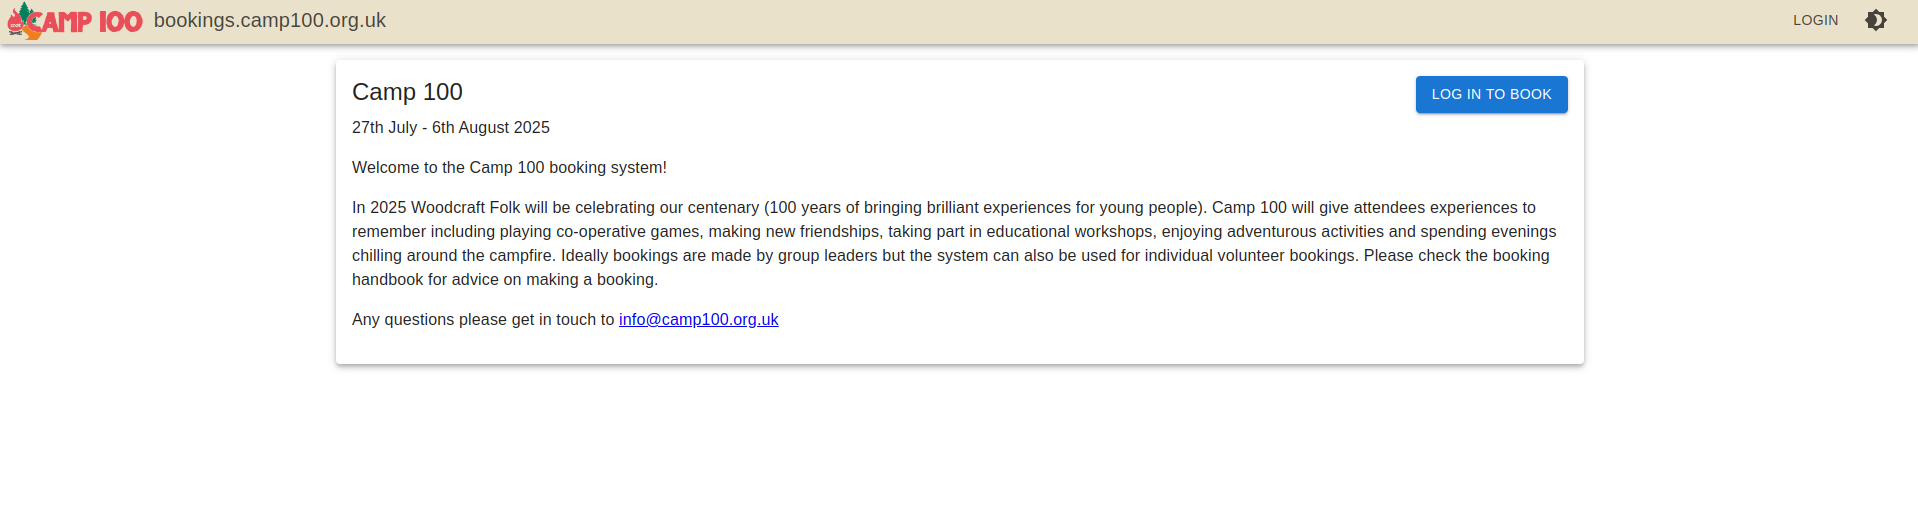
\includegraphics[width=0.9\textwidth]{assets/1-homepage.png}
        \caption{P\'agina de inicio de sistemas de reservas}
    \end{figure}
    \item Selecciona uno de los m\'etodos para iniciar la sesi\'on.
    \begin{figure}[H]
        \centering
        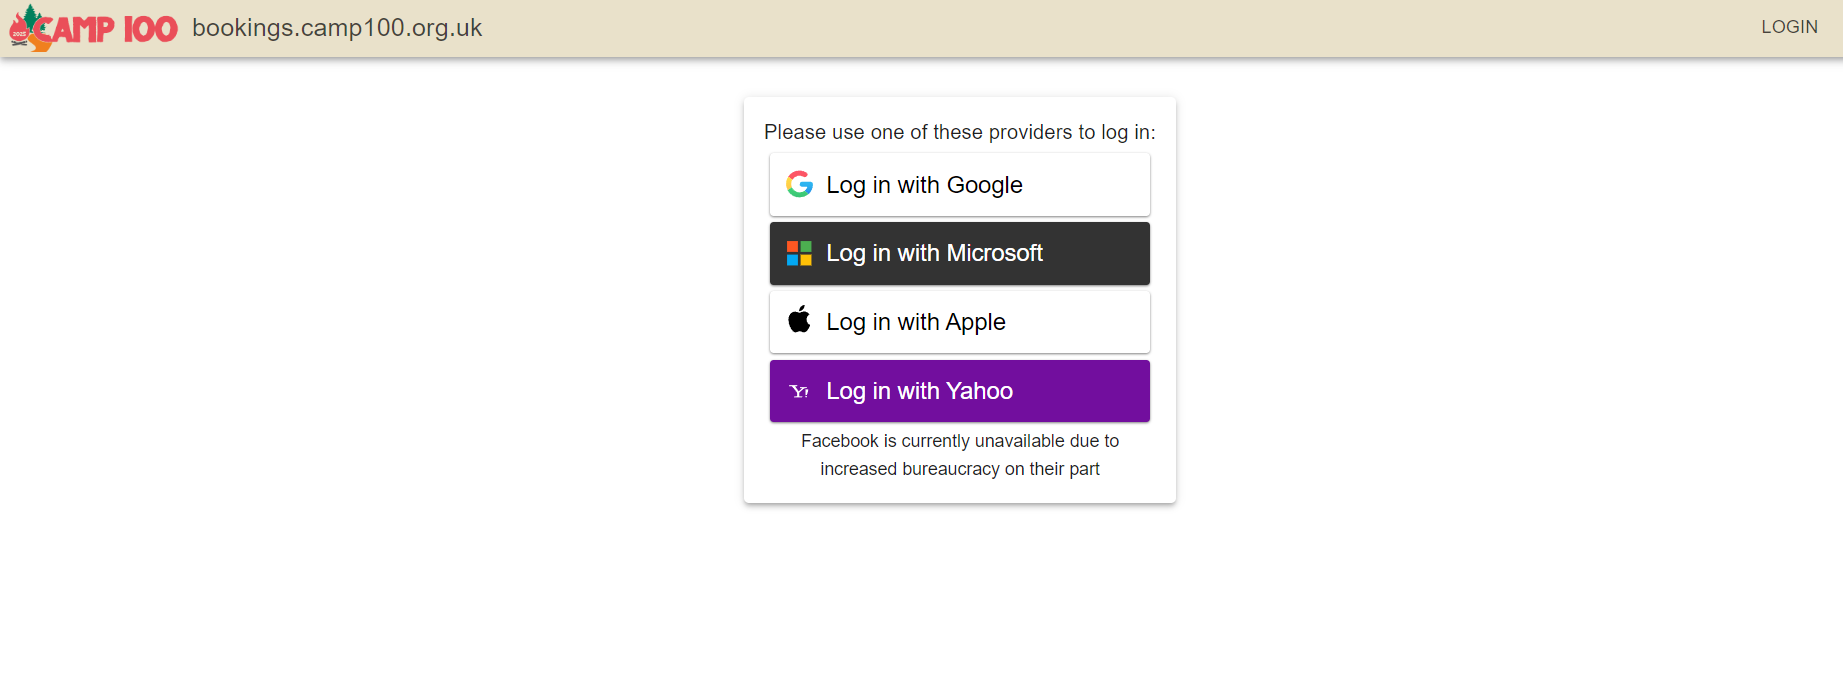
\includegraphics[width=0.9\textwidth]{assets/1-login.png}
        \caption{Opciones de inicio de sesi\'on}
    \end{figure}
    \item Sigue las instrucciones que aparecen en pantalla para iniciar sesi\'on utilizando el m\'etodo que elijas.
    \item Una vez que hayas iniciado sesi\'on, se te redirigir\'a a la pantalla que aparece a continuaci\'on. Tu nombre (o el de la cuenta que est\'es utilizando) aparecer\'a en la esquina superior derecha. Introduce tu nombre y vuelve a introducir tu direcci\'on de correo electr\'onico, haz clic en ``Save'' (guardar).
    \begin{figure}[H]
        \centering
        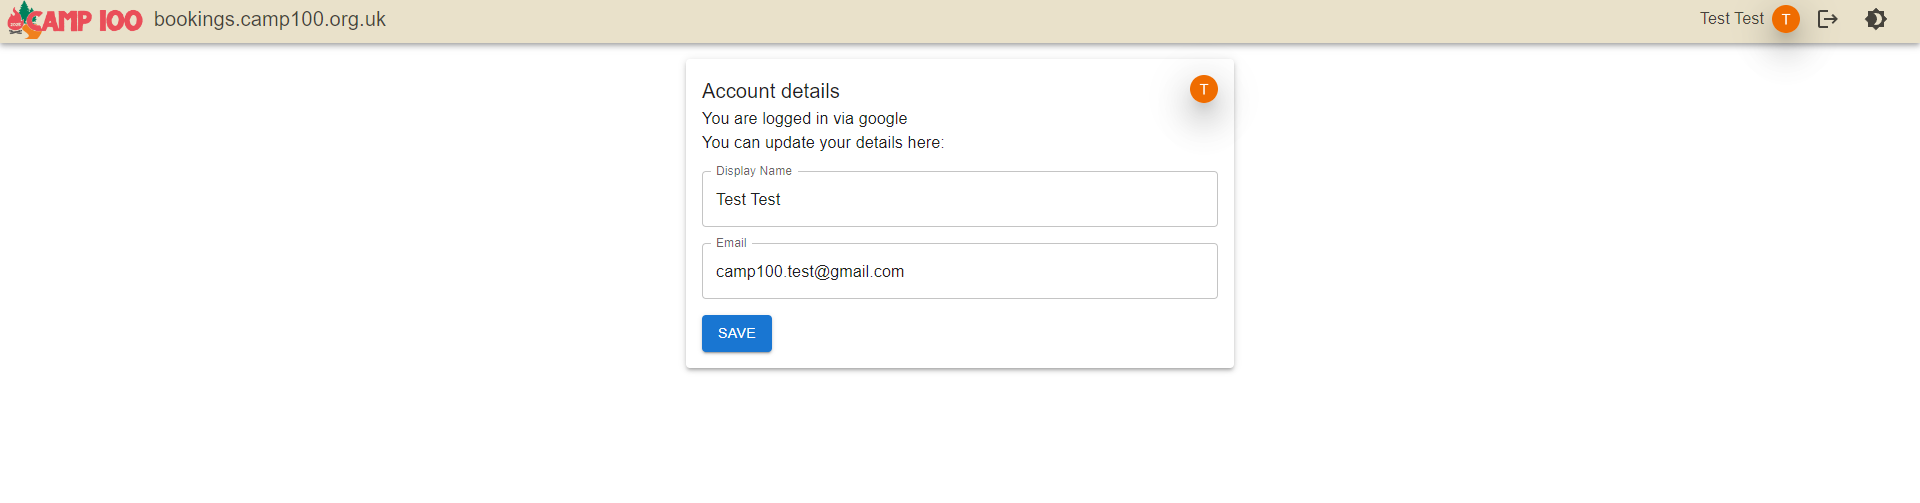
\includegraphics[width=0.9\textwidth]{assets/1-create-account.png}
        \caption{Opciones para crear una cuenta}
    \end{figure}
    \item Se te redirigir\'a a la p\'agina de inicio. Haz clic en ``apply to book'' (solicitar reserva)
    \begin{figure}[H]
        \centering
        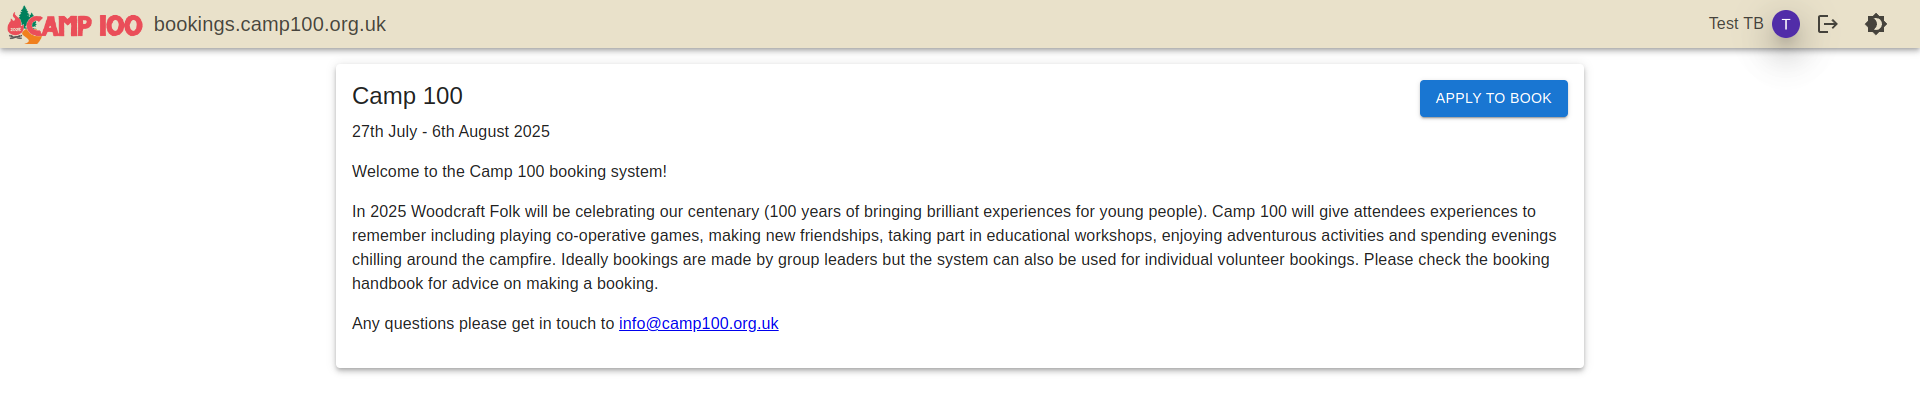
\includegraphics[width=0.9\textwidth]{assets/1-homepage-loggedin.png}
        \caption{Bot\'on Aplicar para reservar}
    \end{figure}
    \item Marca tu reserva es de grupo o individual. Quiz\'as tengas que volver a introducir tu nombre y correo electr\'onico. Selecciona tu organizaci\'on en el men\'u desplegable e introduce el n\'umero aproximado de personas que tienes previsto traer en el cuadro de texto cuando se te solicite y, a continuaci\'on, pulsa ``Submit'' (enviar). (No te preocupes si este dato cambia, lo que necesitamos es hacernos una idea de los n\'umeros.) 
    \begin{figure}[H]
        \centering
        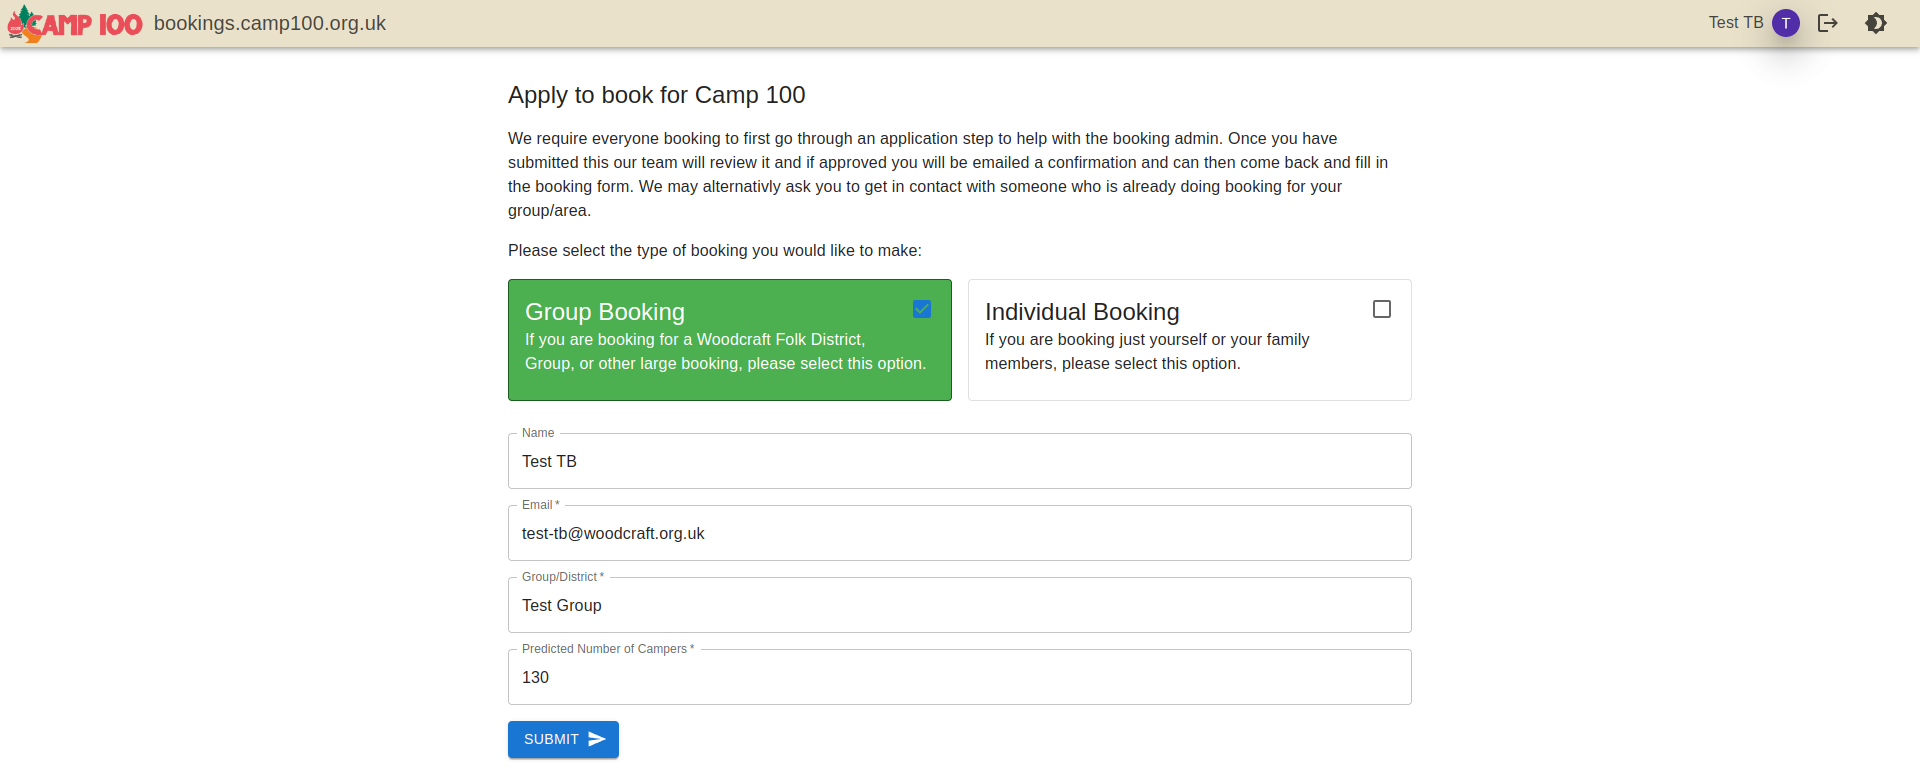
\includegraphics[width=0.9\textwidth]{assets/1-apply.png}
        \caption{P\'agina de solicitud de reserva}
    \end{figure}
    \item Tu solicitud se enviar\'a al equipo de Camp 100
    \item Recibir\'as otro correo electr\'onico cuando tu reserva haya sido aprobada. Pasa a la  \internallink{chap:booking}{Fase 2: Reserva}. Si de tu solicitud se deduce que otra persona del mismo grupo ya ha solicitado reservar, es posible que nos pongamos en contacto contigo para decirte que hables con elle, en lugar de autorizarte a reservar por separado.
\end{enumerate}



\chapter{Fase 2: Reserva}
\label{chap:booking}

Este apartado se refiere a la fase posterior a la autorizaci\'on de tu reserva. Si no tienes claro a qu\'e se refiere la autorizaci\'on de la reserva, consulta la \internallink{chap:apply}{False 1: Solicitud de reserva}.

El sistema de reservas est\'a configurado para ser un sistema ``en tiempo real''. Para facilitar al m\'aximo las cosas a los responsables de grupo, te aconsejamos que a\~nadas a los participantes lo antes posible (incluso mientras el proceso de reserva de tu distrito/grupo local est\'e a\'un abierto). Esto te permitir\'a introducir la informaci\'on poco a poco y proporcionar\'a al equipo de Camp 100 una buena idea del n\'umero de participantes. 

\begin{enumerate}
    \item Ve al \href{https://bookings.camp100.org.uk}{Sistema de reserva de Camp 100}
    \item Haz clic en ``iniciar sesi\'on para reservar''. Comprueba que inicias sesi\'on utilizando el mismo servicio que utilizaste la \'ultima vez (esto es muy importante porque, de lo contrario, tendr\'as que volver a solicitar la reserva).
    \begin{figure}[H]
        \centering
        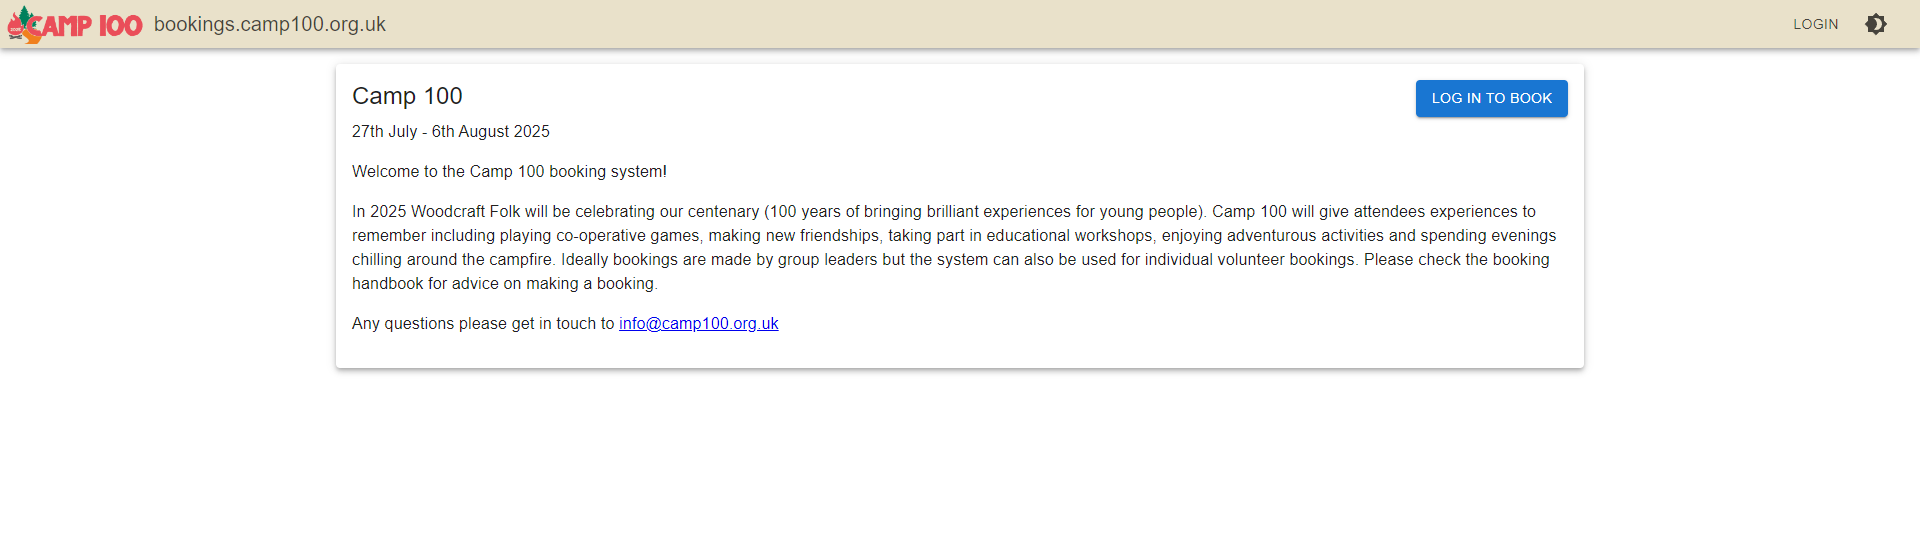
\includegraphics[width=0.9\textwidth]{assets/2-home-prelogin.png}
        \caption{P\'agina de inicio del sistema de reservas}
    \end{figure}
    \item Se te redirigir\'a a la p\'agina de inicio. Haz clic en `Book' (reservar).
    \begin{figure}[H]
        \centering
        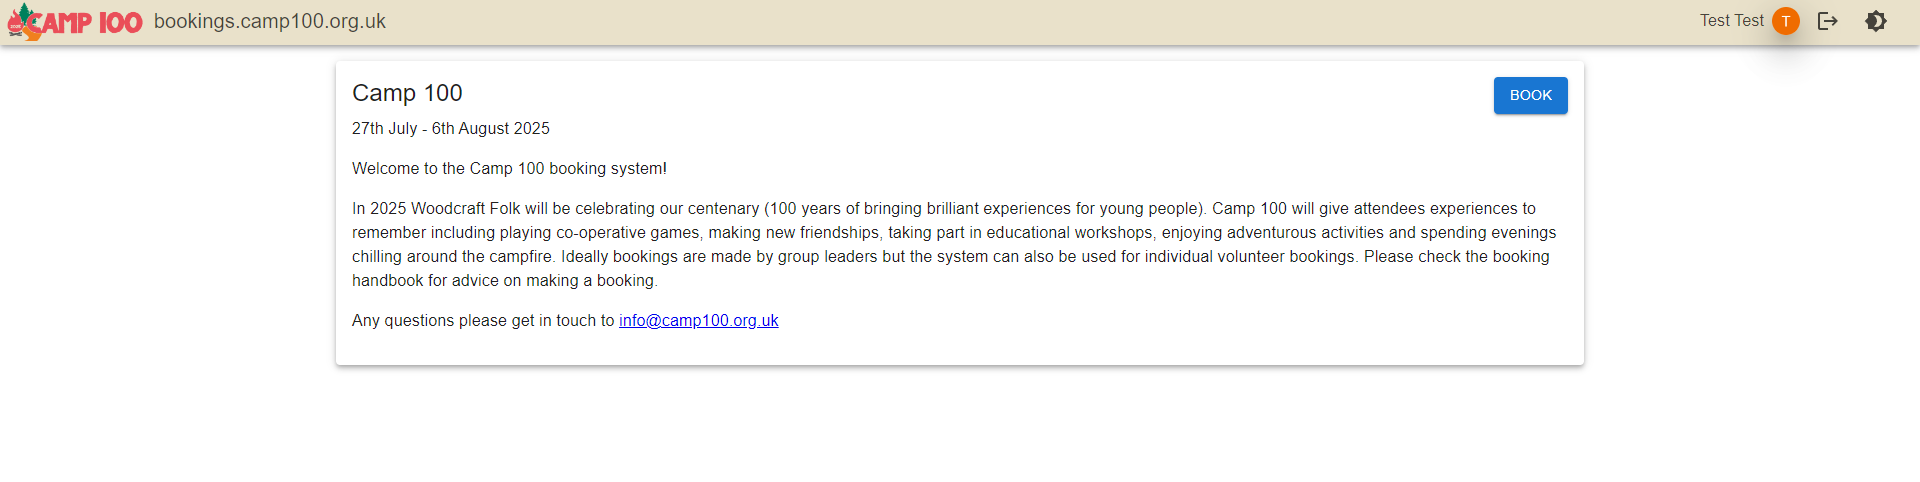
\includegraphics[width=0.9\textwidth]{assets/2-home-loggedin.png}
        \caption{P\'agina de inicio que muestra el bot\'on `Reservar'}
    \end{figure}
    \item Ahora deber\'as introducir algunos datos sobre la reserva. Introduce la informaci\'on en los Recuadros correspondientes. Aqu\'{\i} tendr\'as podr\'as a\~nadir contactos adicionales (opci\'on ``Extra contacts''), que deber\'an ser voluntaries de tu reserva. El equipo de Camp 100 podr\'a ponerse en contacto con cualquier persona de esta lista y contigo para informaros sobre cualquier cuesti\'on sobre el campamento.    
    \item Despl\'azate hacia abajo hasta ``Campers'' (participantes).
    \item Hemos a\~nadido una opci\'on para rellenar los formularios de reserva en una hoja de c\'alculo en lugar de utilizar formularios individuales en el sistema para cada participante. Deber\'as elegir si quieres introducir los datos a trav\'es de una hoja de c\'alculo de Google \textbf{O} completar la reserva utilizando los formularios del sistema de reservas.     
    Si \textbf{NO} vas a utilizar la opci\'on de hoja de c\'alculo \internallink{manual-import}{Pasa \ref*{manual-import}}

    Instrucciones para rellenar la hoja de c\'alculo:
    \begin{enumerate}
        \item Podemos crear una hoja de Google para que la rellenes y luego importar los datos. Es probable que esta sea la opci\'on m\'as sencilla para los grupos grandes. Al hacer clic en el bot\'on ``create sheet'' (crear hoja) se crear\'a una Hoja de Google que se compartir\'a con el correo electr\'onico que hayas indicado. La hoja de c\'alculo te solicitar\'a la misma informaci\'on que el sistema de reservas.  
        
        \textbf{AVISO: Al importar los datos desde la hoja de c\'alculo se sobrescribir\'an aquellos que ya hayas introducido en los formularios del sistema de reservas, por lo que es importante que elijas el m\'etodo que vas a utilizar.}
        \begin{figure}[H]
            \centering
            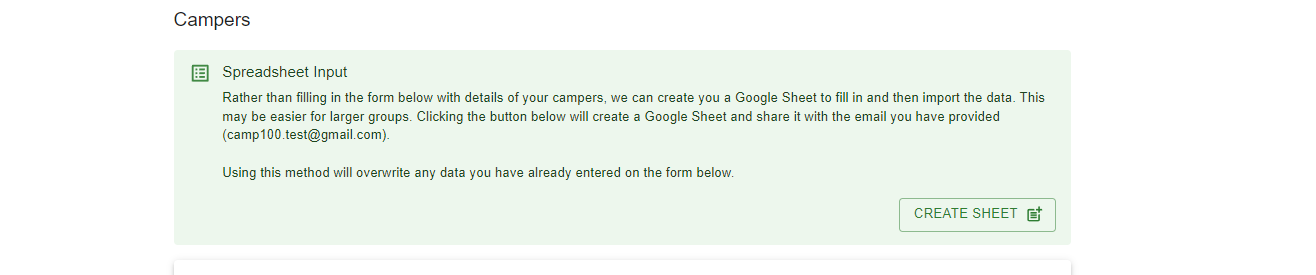
\includegraphics[width=0.9\textwidth]{assets/2-spreadsheet-option.png}
            \caption{Bot\'on Crear hoja}
        \end{figure}
        \item Una vez que hayas creado la hoja de c\'alculo, recibir\'as un correo electr\'onico con un enlace a \'esta en la direcci\'on con la que hiciste la reserva. Para acceder a la hoja de c\'alculo necesitar\'as tener una cuenta de Google (puedes crear una cuenta de Google incluso sin tener una direcci\'on de correo electr\'onico de Gmail, aqu\'{\i} encontrar\'as ayuda - \href{https://support.google.com/accounts/answer/27441?hl=es}{support.google.com/accounts/answer/27441?hl=es} ) 
        \item Una vez que hayas recibido el correo electr\'onico, podr\'as abrir la hoja de c\'alculo de Google desde el enlace.
         \begin{figure}[H]
            \centering
            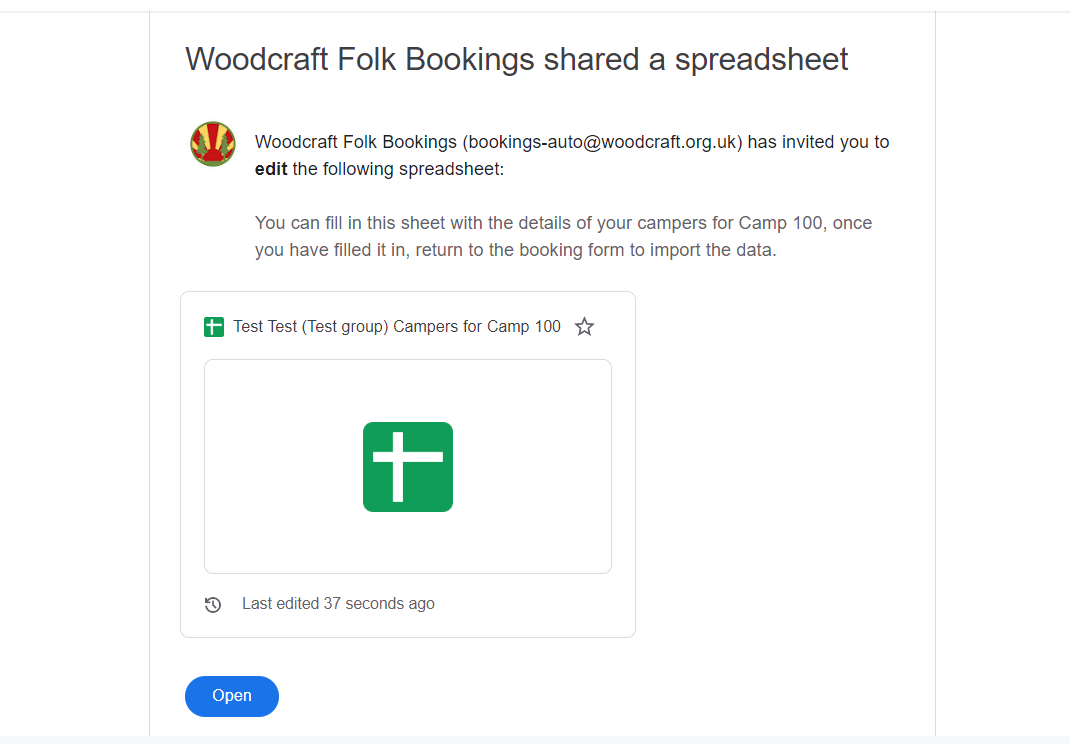
\includegraphics[width=0.6\textwidth]{assets/2-spreadsheet-email.png}
            \caption{Correo electr\'onico que muestra la hoja de c\'alculo compartida}
        \end{figure}
        \item Cuando abras la hoja de c\'alculo ver\'as los mismos campos que en los formularios del sistema de reservas. Te recomendamos que compartas el  \internallink{chap:template-booking-form}{ejemplo de formulario} que figura al final de esta gu\'{\i}a con las madres/ padres/cuidadores de tu grupo y utilices esa informaci\'on para introducir los datos de cada participante en la hoja de c\'alculo. Necesitaremos una direcci\'on de correo electr\'onico para cada participante; si se trata de une menor de 16 a\~nos, deber\'a tratarse del correo electr\'onico de uno de sus madres, padres o tutores, y para los mayores de 16 a\~nos, una direcci\'on de correo electr\'onico personal, siempre que sea posible. Utilizaremos esta informaci\'on para comunicar a les participantes o a sus madres, padres o tutores la informaci\'on m\'as importante y comprobar la afiliaci\'on a Woodcraft Folk.
        \begin{figure}[H]
            \centering
            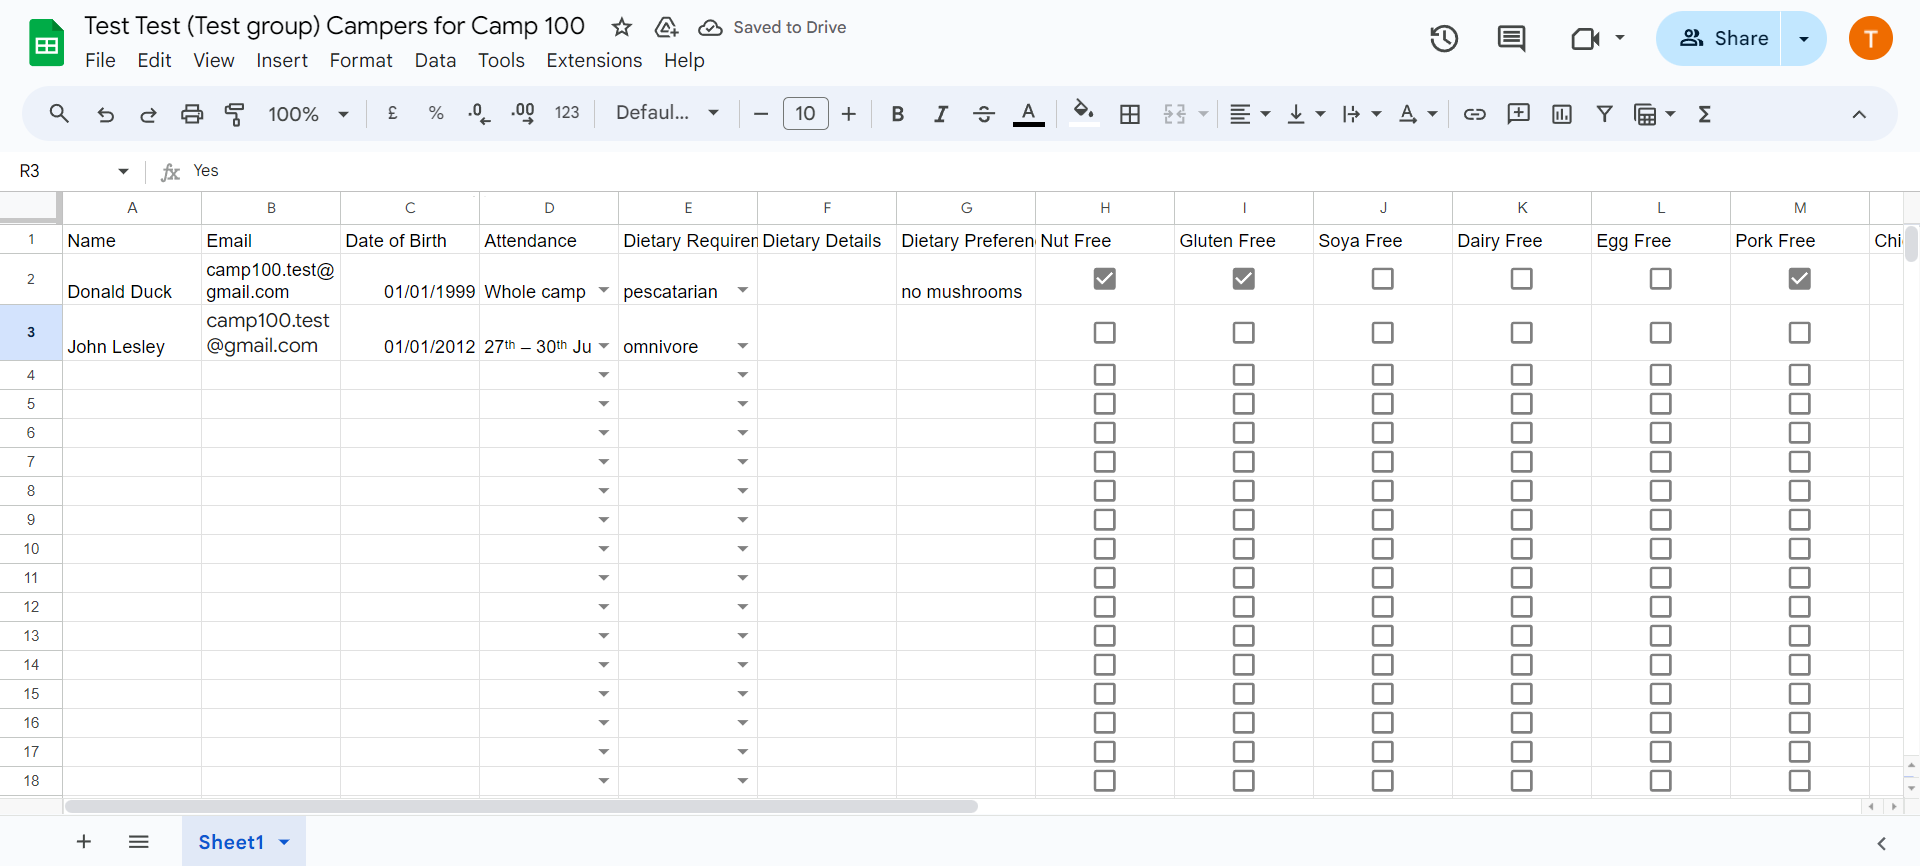
\includegraphics[width=0.9\textwidth]{assets/2-spreadsheet.png}
            \caption{Hoja de c\'alculo que muestra informaci\'on de los campistas de ejemplo}
        \end{figure}
        \item Podr\'as volver a la hoja de c\'alculo y actualizarla, a\~nadir nueves participantes y eliminarles en cualquier momento antes de la fecha l\'{\i}mite de reserva. Todos los cambios se guardar\'an autom\'aticamente en la hoja de Google. Puedes importar los datos al sistema de reservas en cualquier momento volviendo al sistema de reservas y haciendo clic en ``import data'' (importar datos).\textbf{AVISO: Al importar los datos desde la hoja de c\'alculo se sobrescribir\'an aquellos que ya hayas introducido en los formularios del sistema de reservas. }
        \begin{figure}[H]
            \centering
            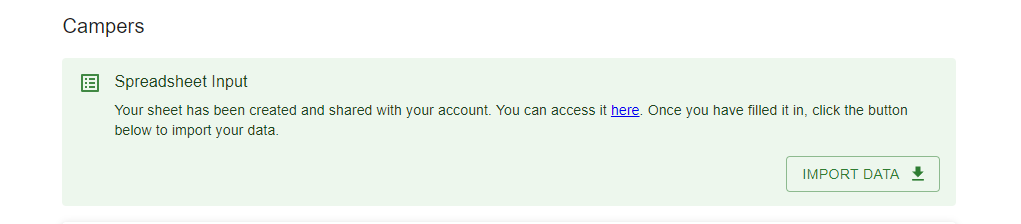
\includegraphics[width=0.9\textwidth]{assets/2-spreadsheet-import.png}
            \caption{Bot\'on `Importar datos'}
        \end{figure}
        \item Una vez importados tus datos, la informaci\'on de los participantes se rellenar\'a en los campos de los formularios del sistema de reservas. Los participantes aparecer\'an en la parte derecha de la pantalla, lo que te ayudar\'a a llevar un registro de tu reserva.
        \begin{figure}[H]
            \centering
            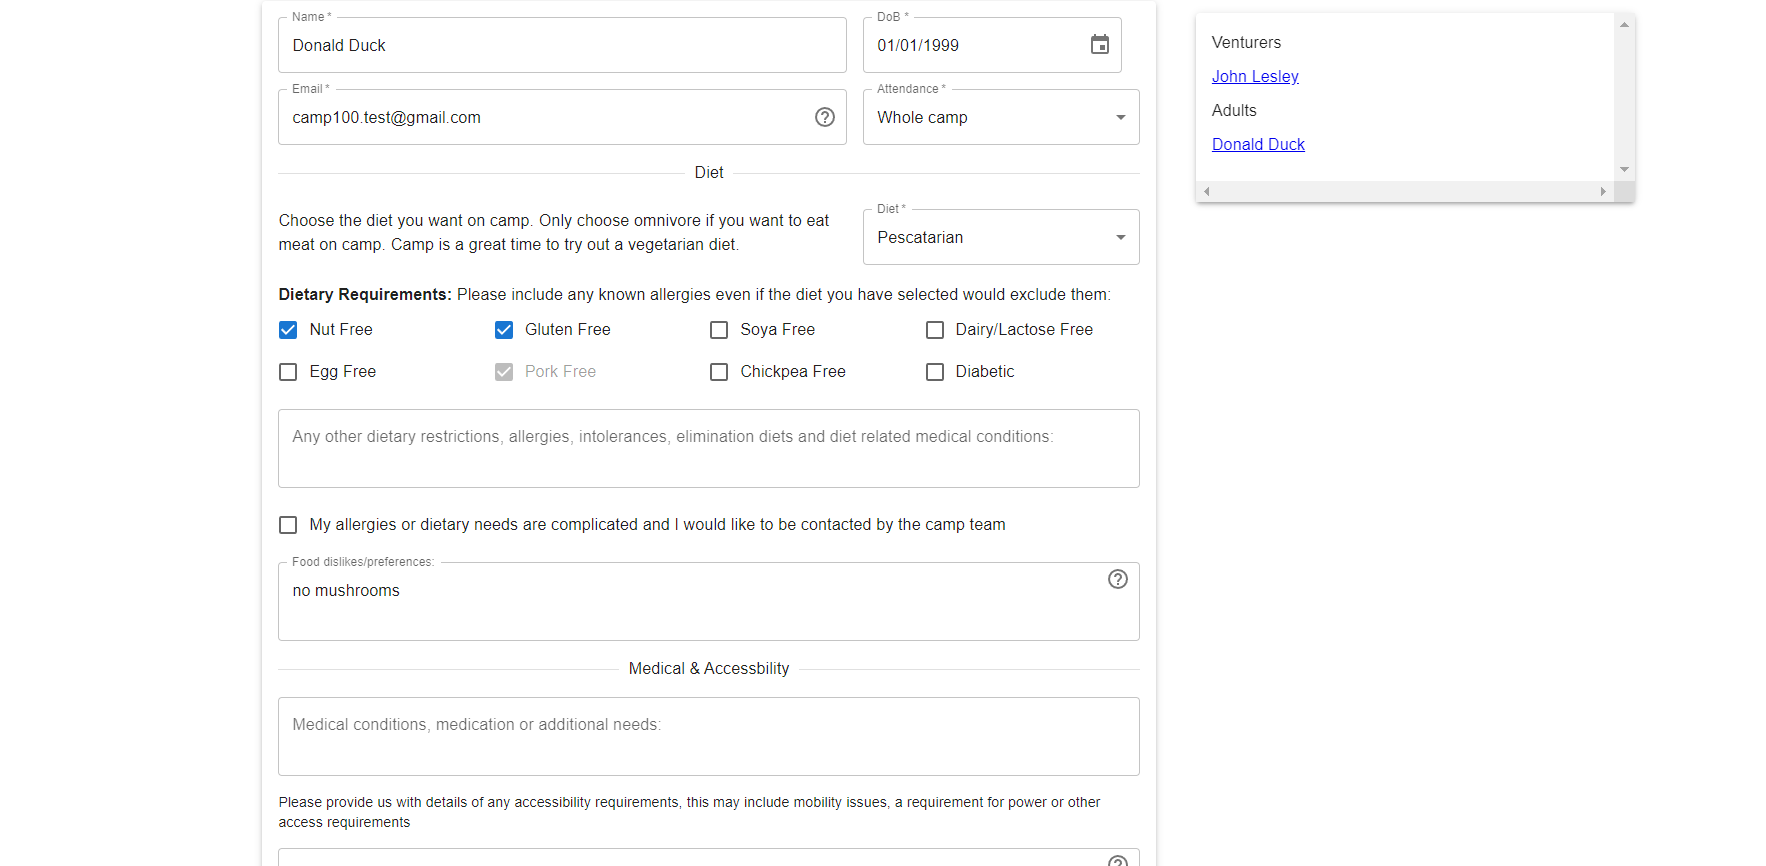
\includegraphics[width=0.9\textwidth]{assets/2-spreadsheet-review.png}
            \caption{Data imported from the spreadsheet show on the booking system}
        \end{figure}
        \item Una vez que hayas importado los datos de la hoja de c\'alculo, deber\'as completar el resto del formulario y enviarlo. \internallink{everyone-steps}{Pasa directamnete al paso \ref*{everyone-steps}} para finalizar tu reserva.
    \end{enumerate}
    \item \label{manual-import}  Si no utilizas la hoja de c\'alculo, deber\'as rellenar el siguiente formulario por cada participante. Una vez a\~nadidos, los participantes aparecer\'an en la parte derecha de la pantalla, lo que te ayudar\'a a llevar un registro de tu reserva. Necesitaremos una direcci\'on de correo electr\'onico para cada participante; si se trata de une menor de 16 a\~nos, deber\'a tratarse del correo electr\'onico de uno de sus madres, padres o tutores, y para los mayores de 16 a\~nos, una direcci\'on de correo electr\'onico personal, siempre que sea posible. Utilizaremos esta informaci\'on para comunicar a les participantes o a sus madres, padres o tutores la informaci\'on m\'as importante y comprobar la afiliaci\'on a Woodcraft Folk.

    \begin{figure}[H]
        \centering
        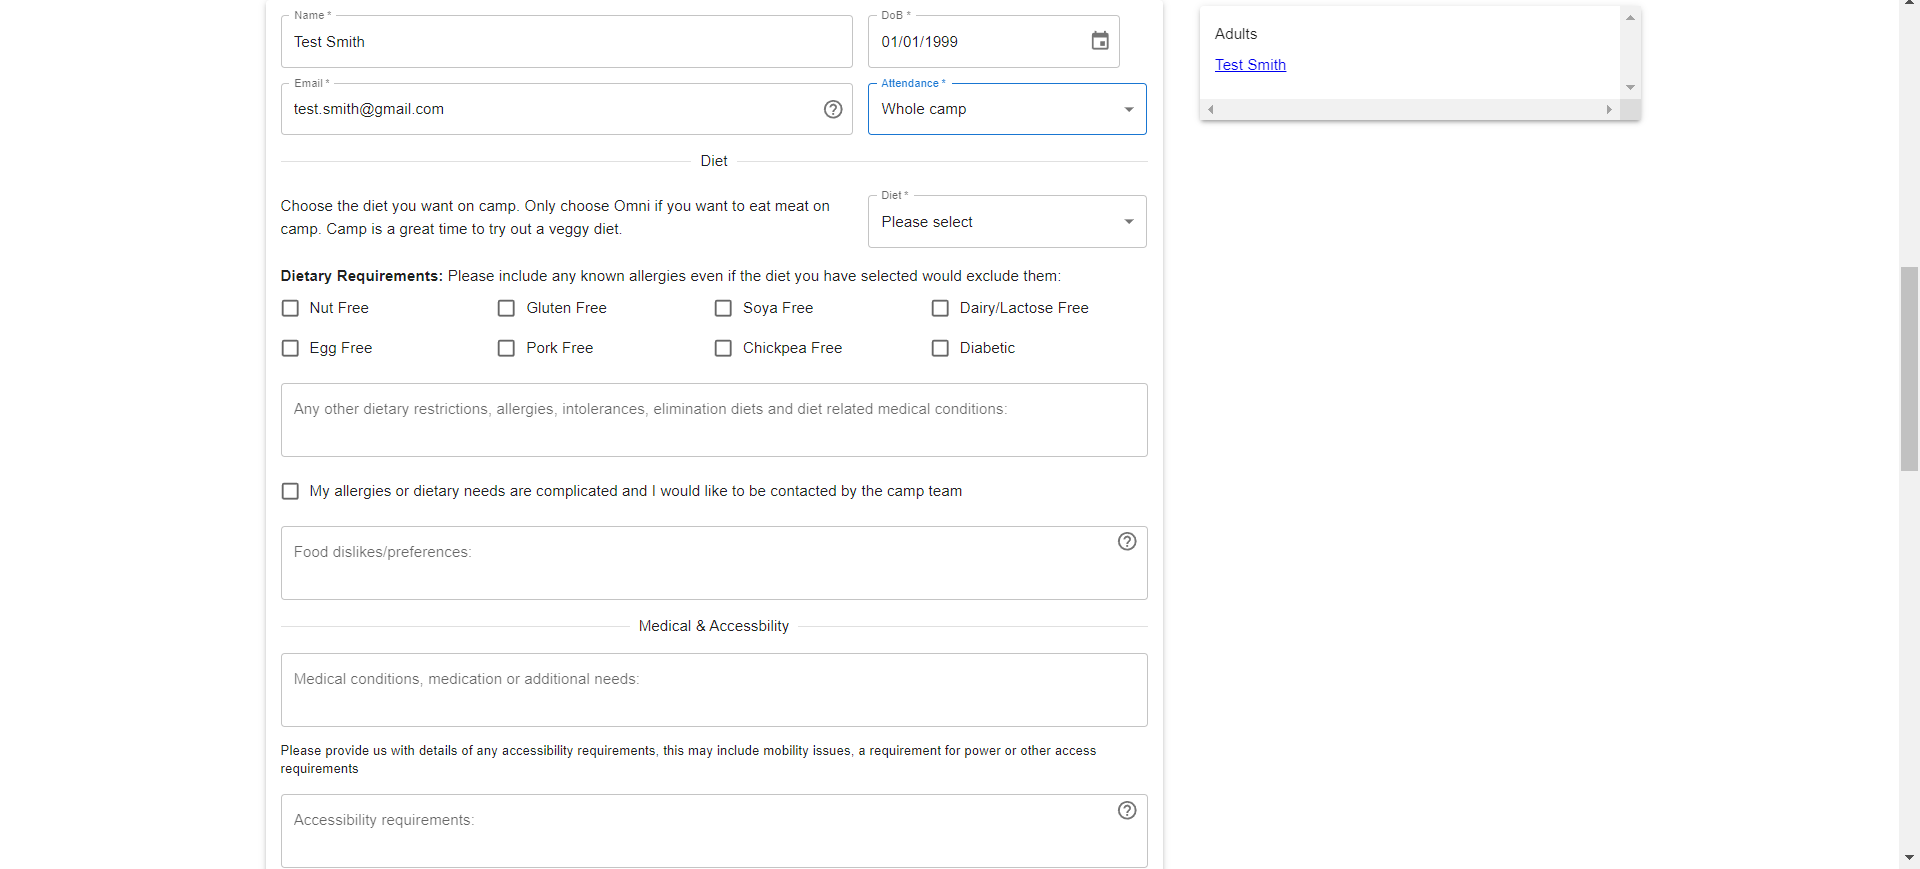
\includegraphics[width=0.9\textwidth]{assets/2-manual-input.png}
        \caption{Ingresar manualmente un participante}
    \end{figure}
    \item Para a\~nadir m\'as participantes, haz clic en el bot\'on `Add Person' (a\~nadir persona). Esto a\~nadir\'a otro formulario en blanco para rellenar.
    \item Para eliminar a une participante, haz clic en el bot\'on naranja con forma de candado para `desbloquear' el bot\'on de eliminar y, a continuaci\'on, en el bot\'on con forma de cruz que aparece junto a \'el.
    \begin{figure}[H]
        \centering
        
\includegraphics[width=0.9\textwidth]{assets/2-add-person-button.png}
        \caption{Bot\'on `Agregar persona' y candado naranja}
    \end{figure}
    \item \label{everyone-steps}Una vez que hayas introducido la informaci\'on de todos tus participantes, despl\'azate hasta el apartado `Camping' (acampada). Introduce aqu\'{\i} cualquier informaci\'on relevante sobre con qu\'e otros grupos te gustar\'{\i}a acampar, de qu\'e equipo dispones y sobre cualquier necesidad de acceso de tus participantes. Aqu\'{\i} puedes incluir las necesidades de acceso de los participantes que a\'un no se han inscrito, pero que prev\'es que asistir\'an al campamento.  
    \item Despl\'azate hasta abajo hasta «Money» (dinero). Aqu\'{\i} podr\'as ver un desglose del coste de tu grupo para 
    venir al campamento, tu referencia de pago que ser\'a C100-XXXXX (que deber\'a utilizarse para todos los pagos) e instrucciones de pago. Si alguno de los miembros de tu grupo solicita una contribuci\'on del fondo de acceso, te informaremos por correo electr\'onico de si la hab\'eis obtenido y modificaremos en tal caso el importe adeudado en el sistema. Para m\'as informaci\'on sobre el pago, consulta el 
    \internallink{chap:payment}{apartado \ref*{chap:payment}}. 
    \begin{figure}[H]
        \centering
        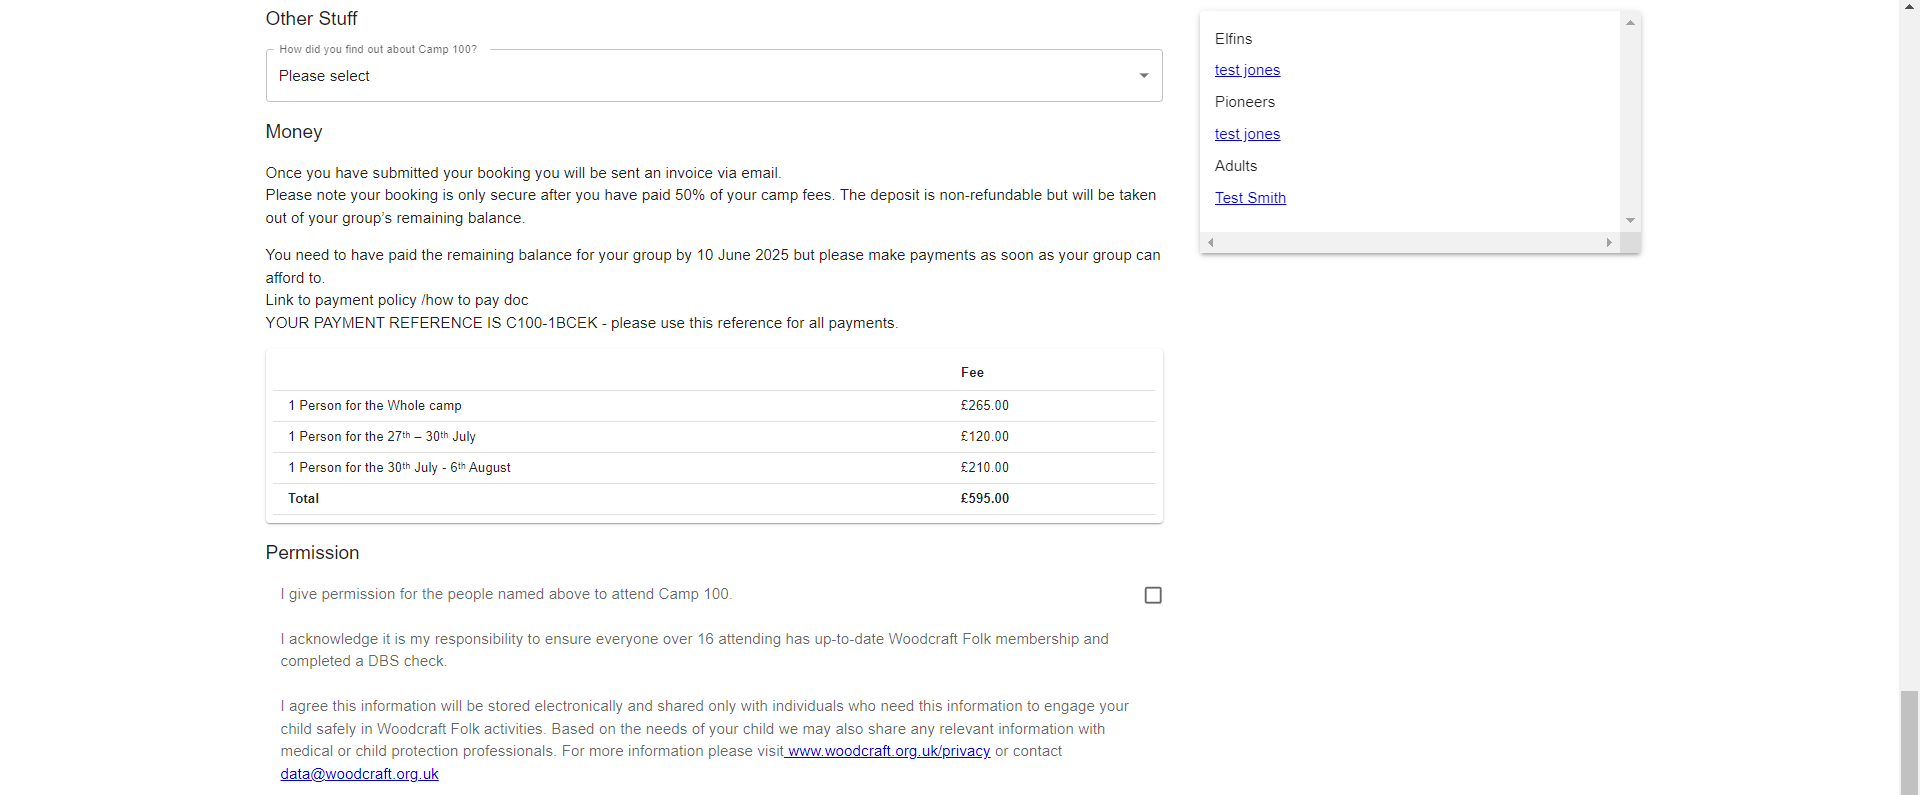
\includegraphics[width=0.9\textwidth]{assets/2-money.png}
        \caption{Secci\'on `Dinero'}
    \end{figure}
    \item Contin\'ua desplaz\'andote para abajo. Para las reservas individuales, deber\'as a\~nadir los datos de un mayor de 16 a\~nos que pueda actuar como contacto de emergencia. Esto se hace en el apartado `Emergency Contact' (contacto de emergencia).
    \item Autoriza la asistencia y reconoce la responsabilidad y, a continuaci\'on, env\'{\i}a la reserva. Llegar\'as a una pantalla en la que se confirmar\'a la informaci\'on sobre los precios y un resumen de la reserva. Tambi\'en recibir\'as un correo electr\'onico de confirmaci\'on con la factura de tu reserva, que se modificar\'a y reenviar\'a cada vez que modifiques tu reserva. 
    \begin{figure}[H]
        \centering
        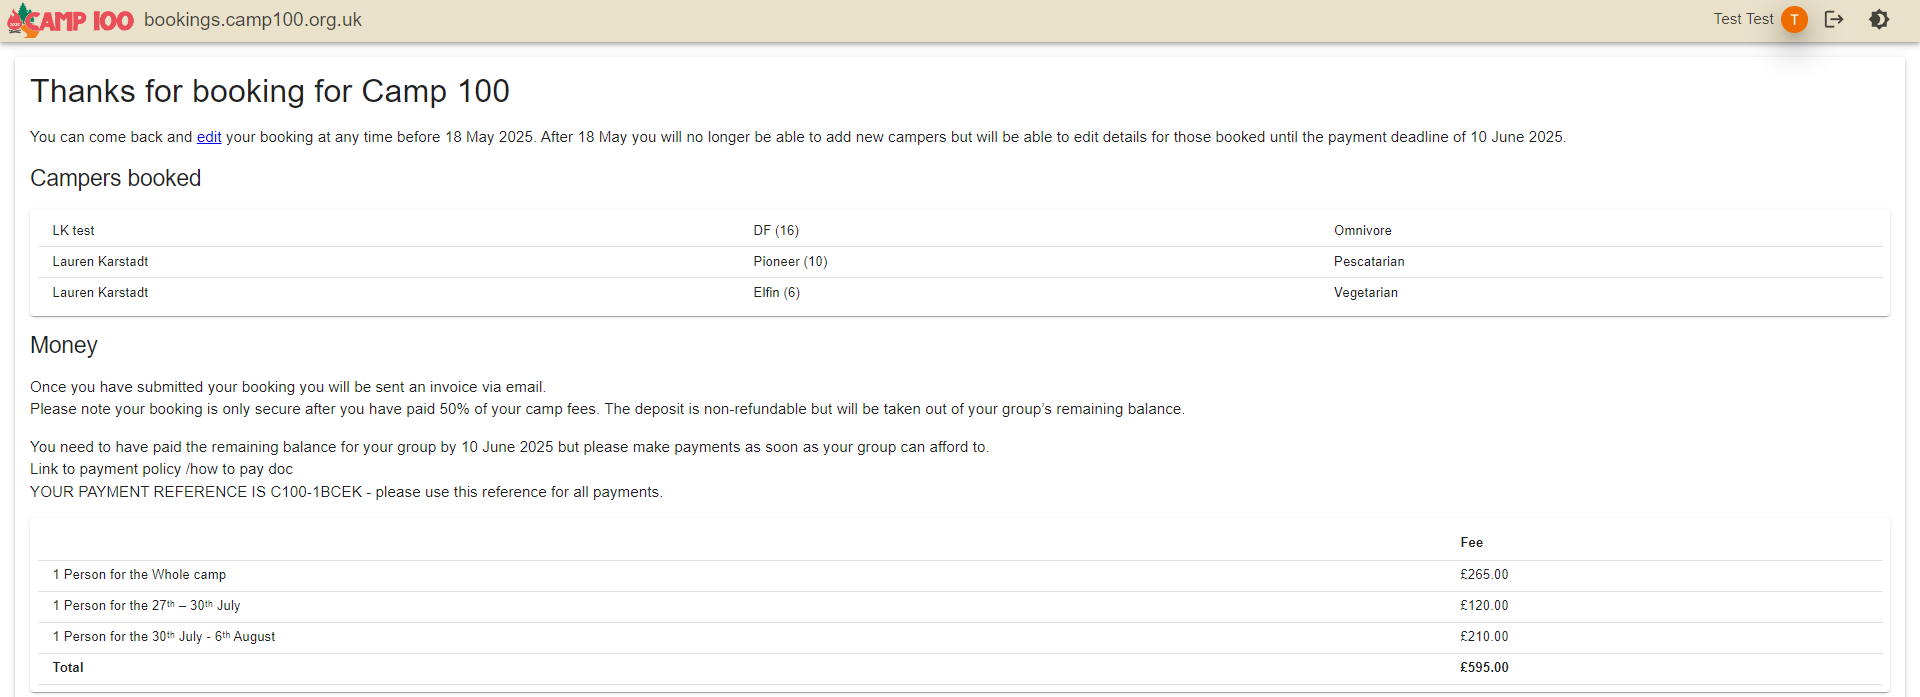
\includegraphics[width=0.9\textwidth]{assets/2-booking-confirmation.png}
        \caption{P\'agina de confirmaci\'on de reserva}
    \end{figure}
    
\end{enumerate}


\chapter{Fase 3: Modificar tu reserva}
\label{chap:edit}

Es normal que quieras a\~nadir m\'as informaci\'on o m\'as personas a tu reserva cuando se acerque el Camp 100. 

Puedes modificar tu reserva tantas veces como desees hasta el \textbf{18 de mayo de 2025.}. Despu\'es de esta fecha no podr\'as a\~nadir nuevos participantes, pero podr\'as modificar tu reserva si se produce alg\'un cambio, aunque no podemos asegurar que podamos realizar cambios o reembolsos despu\'es de esta fecha. El \'ultimo plazo de pago para el Camp 100 es el 10 de junio de 2025, despu\'es de esta fecha tendr\'as que hablar con el personal de Woodcraft Folk para modificar tu reserva. 
 
\begin{enumerate}
    \item Ve al \href{https://bookings.camp100.org.uk}{Sistema de reserva de Camp 100}
    \item Haz clic en login (iniciar sesi\'on). Comprueba que utilizas el mismo servicio con el que has iniciado sesi\'on anteriormente, ya que de lo contrario tendr\'as que volver a solicitar la reserva.    
    \item La p\'agina de inicio mostrar\'a un resumen de tu reserva y la informaci\'on de pago.
    \item Haz clic en `Edit My Booking' (modificar mi reserva).
    \item Esto te conducir\'a a la misma p\'agina que visitaste cuando hiciste la reserva, donde podr\'as modificar tu reserva en el sistema. Si utilizas el m\'etodo de hoja de c\'alculo para realizar la reserva, puedes actualizar tu hoja de c\'alculo y a\~nadir/eliminar/modificar participantes en cualquier momento antes de la fecha l\'{\i}mite. Recuerda importar los datos al sistema de reservas para que se actualicen tus datos de facturaci\'on y pago.
    \item Una vez que hayas terminado de realizar los cambios, deber\'as volver a marcar la casilla `Permission' (permiso) y luego hacer clic en `Submit booking' (Enviar reserva).
    \item Una vez que hayas enviado tu reserva, recibir\'as por correo electr\'onico un resumen de los Cambios y la factura actualizada.
    
\end{enumerate}

\chapter{Pago}
\label{chap:payment}

\begin{callout-orange}{M\'as informaci\'on}
    La pol\'{\i}tica de pago y la informaci\'on completa sobre c\'omo pagar se pueden encontrar en \href{https://camp100.org.uk}{La pol\'{\i}tica de pago y la informaci\'on completa sobre c\'omo pagar se pueden encontrar en el sitio web de Camp 100}
\end{callout-orange}

Una vez que hayas realizado la reserva, se te asignar\'a una referencia. Tendr\'a el siguiente formato C100-XXXXX, (en lugar de XXXXX aparecer\'a un c\'odigo aleatorio).
Esta referencia permite identificar de forma \'unica tu reserva. Deber\'as utilizarla al realizar el pago de modo que podamos identificar que proviene de ti y descontarlo de tu saldo pendiente.


\section{Pagos en el Reino Unido}

Por favor transfiera todos los pagos a la siguiente cuenta\\
\textbf{Titular de la cuenta:} Woodcraft Folk\\
\textbf{No. de cuenta:} 2039 2756\\
\textbf{Sucursal:} 60 83 01

Comprueba la referencia \'unica en la confirmaci\'on de tu reserva, es decir C100-XXXXX. Recuerda utilizar esta referencia para la fianza y todos los pagos posteriores. 

Si por cualquier motivo no puedes a\~nadir una referencia, env\'{\i}anos un correo electr\'onico a info@camp100.org.uk e ind\'{\i}canos el importe y la fecha de pago y para qui\'en se refer\'{\i}a. As\'{\i} podremos vincularlo a tu reserva y poner al d\'{\i}a tu registro de pagos.


\section{Pagos internacionales}

Por favor transfiera todos los pagos a la siguiente cuenta\\
\textbf{Swift Code (BIC):} NWBKGB2L\\
\textbf{N\'umero IBAN:} GB93NWBK60023571418024\\
\textbf{Direcci\'on de la organizaci\'on:} \\
Holyoake House, Hanover Street, Manchester, M60 0AS, Reino Unido

Comprueba la referencia \'unica en la confirmaci\'on de tu reserva, es decir C100-XXXXX. Recuerda utilizar esta referencia para la Fianza y todos los pagos posteriores. 

Si por cualquier motivo no puedes a\~nadir una referencia, env\'{\i}anos un correo electr\'onico a info@camp100.org.uk e ind\'{\i}canos el importe que pagaste, la fecha de pago y para qui\'en. As\'{\i} podremos vincularlo a tu reserva y poner al d\'{\i}a tu registro de pagos.



\chapter[Modelo de formulario de reserva]{Modelo de\\ formulario de reserva}
\label{chap:template-booking-form}

Hemos elaborado un modelo de formulario de reserva para que los responsables de grupo recopilen informaci\'on sobre los miembros de su grupo antes de introducirla en el sistema de reserva.
Algunos de los datos que figuran a continuaci\'on sirven s\'olo como referencia para el distrito/grupo y no se solicitan a nivel central, por lo que te recomendamos que guardes estos formularios para informaci\'on como, en caso de emergencia, los datos del m\'edico, etc.  La hemos incluido a continuaci\'on \'unicamente como referencia \href{https://drive.google.com/file/d/1oSFIkZQxzes3VTi5ZqPHCcAu4DiscvOm/view}{Aqu\'{\i}} podr\'as descargar una copia editable. 

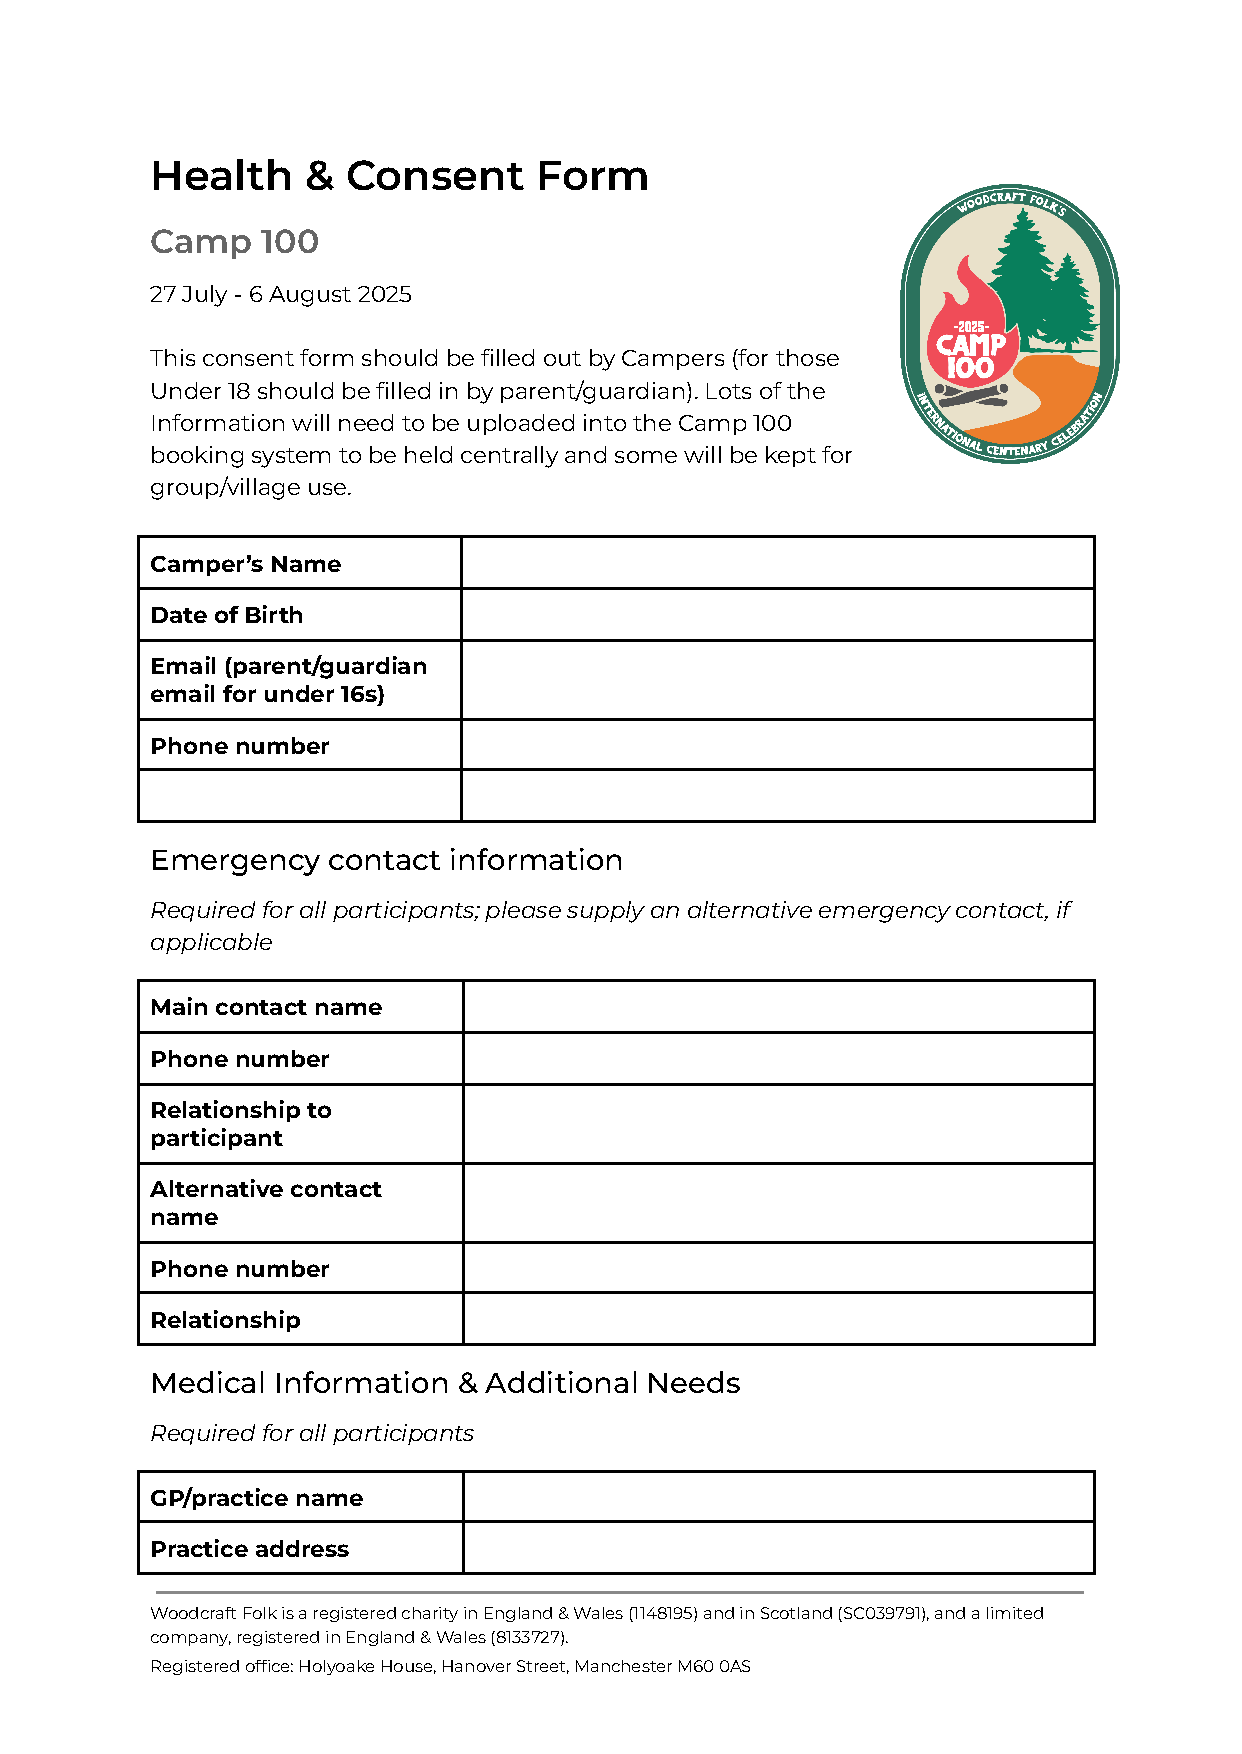
\includepdf[pagecommand={\pagestyle{fancy}}, scale=0.8, pages=-, frame]{assets/template-consent-form.pdf}

\makedocumentbackpage

\end{document}